% Digital Campus - Internship Report (Summer 2026)
% Compile with pdfLaTeX (e.g. on Overleaf). Modern, clean LaTeX styling.
\documentclass[11pt,a4paper]{article}

\usepackage[T1]{fontenc}
\usepackage[utf8]{inputenc}
\usepackage{lmodern}
\usepackage[a4paper,margin=2.3cm]{geometry}
\usepackage[dvipsnames,table]{xcolor}
\usepackage{titlesec}
\usepackage{booktabs}
\usepackage{array}
\usepackage{tabularx}
\usepackage{enumitem}
\usepackage{fancyhdr}
\usepackage{graphicx}
\usepackage[most]{tcolorbox}
\usepackage{tikz}
\usetikzlibrary{arrows.meta,positioning}
\usepackage[hidelinks]{hyperref}

% ---- palette ----
\definecolor{navy}{HTML}{0F172A}
\definecolor{brandblue}{HTML}{1D4ED8}
\definecolor{brandblue2}{HTML}{2563EB}
\definecolor{ink}{HTML}{1F2937}
\definecolor{slate}{HTML}{475569}
\definecolor{light}{HTML}{EFF6FF}
\definecolor{rule}{HTML}{DBEAFE}
\definecolor{green}{HTML}{16A34A}

\hypersetup{colorlinks=true, linkcolor=brandblue, urlcolor=brandblue}

% ---- section styling (sans, colored) ----
\titleformat{\section}{\color{navy}\sffamily\LARGE\bfseries}{\thesection.}{0.5em}{}
\titleformat{\subsection}{\color{brandblue}\sffamily\large\bfseries}{\thesubsection}{0.5em}{}
\titlespacing*{\section}{0pt}{18pt}{8pt}

% ---- header / footer ----
\pagestyle{fancy}\fancyhf{}
\renewcommand{\headrulewidth}{0.4pt}
\renewcommand{\footrulewidth}{0.4pt}
\fancyhead[L]{\footnotesize\sffamily\color{slate}Digital Campus\,\textbar\,Internship Report 2026}
\fancyhead[R]{\footnotesize\sffamily\color{slate}FSB Nexus}
\fancyfoot[C]{\footnotesize\sffamily\color{slate}\thepage}

% ---- callout box ----
\newtcolorbox{callout}{colback=light,colframe=brandblue,boxrule=0pt,
  leftrule=3pt,arc=2pt,left=8pt,right=8pt,top=6pt,bottom=6pt}
\newtcolorbox{okbox}{colback=green!6,colframe=green,boxrule=0pt,
  leftrule=3pt,arc=2pt,left=8pt,right=8pt,top=6pt,bottom=6pt}

\newcolumntype{Y}{>{\raggedright\arraybackslash}X}
\setlist[itemize]{leftmargin=1.3em,itemsep=2pt,topsep=3pt}

\begin{document}

% ================= TITLE PAGE =================
\begin{titlepage}
\centering
\vspace*{1.4cm}
{\sffamily\bfseries\color{brandblue}\large UNIVERSIT\'E DE CARTHAGE \quad\textbullet\quad FACULT\'E DES SCIENCES DE BIZERTE}\\[4pt]
{\color{rule}\rule{0.42\textwidth}{1.2pt}}\\[26pt]
{\sffamily\bfseries\color{navy}\fontsize{34}{38}\selectfont Digital Campus}\\[10pt]
{\itshape\color{slate}\Large An Intelligent, Source-Grounded Assistant\\ for the Facult\'e des Sciences de Bizerte}\\[18pt]
{\sffamily\large\bfseries Summer Internship Report --- 2026}\\[4pt]
{\sffamily\color{slate} Project codename: \textbf{FSB Nexus}}\\[26pt]

\begin{tabular}{@{}>{\bfseries}p{4.4cm} p{9.6cm}@{}}
\toprule
\multicolumn{1}{@{}l}{\color{navy}\sffamily Team member} & \multicolumn{1}{l}{\color{navy}\sffamily Primary role}\\
\midrule
Aymen Jeddou & RAG intelligent system (Role 1), Scrum Master, branch integration\\[2pt]
Iheb Bouali & Knowledge base; frontend enhancement (\texttt{better\_front})\\[2pt]
Abderrahim Neji & Backend development; Google Classroom integration (Role 2)\\[2pt]
Mohamed Amine Trabelsi & Frontend design, then security \& platform hardening (Role 4)\\
\bottomrule
\end{tabular}

\vspace{22pt}
{\sffamily\color{slate} Academic year 2025--2026}\\[10pt]
{\sffamily\color{slate} Supervisor: \rule{4.5cm}{0.4pt} \quad Internship host: \rule{4.5cm}{0.4pt}}\\[8pt]
{\sffamily\color{slate} Internship period: \rule{6cm}{0.4pt}}
\vfill
\end{titlepage}

\tableofcontents
\thispagestyle{fancy}
\newpage

% ================= 1 =================
\section{Introduction and Context}
Students at the Facult\'e des Sciences de Bizerte (FSB) face a familiar problem: the information they need --- admission conditions, available licences and masters, course prerequisites, the academic calendar, administrative procedures --- is scattered across PDFs, notice boards and word of mouth. General-purpose chatbots answer confidently but invent details, which is worse than no answer at all in an academic setting.

\textbf{Objective.} During the summer 2026 internship, our four-person team built \textbf{Digital Campus} (codename \textit{FSB Nexus}): a web platform whose centrepiece is an \textbf{agentic Retrieval-Augmented Generation (RAG) assistant} that answers questions \textit{only} from official FSB documents and \textbf{cites its sources} on every answer. If the documents do not support an answer, the assistant says so rather than guessing.

\textbf{Scope of this report.} This is a team report. It describes the whole platform, explains how the four of us divided the work, and then goes deeper on each technical area --- with a dedicated chapter on the RAG intelligent system and its measured results. All work described here currently lives on the \texttt{develop} branch and is pending a final merge to \texttt{main}.

\begin{callout}
\textbf{At a glance.} Four layers (frontend, backend, AI/RAG, knowledge base); a multilingual French/Arabic/English assistant; streamed, cited answers; a courses module with Google Classroom import; and a final hardening sprint that added onboarding, server-side access control, rate limiting, database migrations and continuous integration.
\end{callout}

% ================= 2 =================
\section{Project Overview}
Digital Campus is composed of four cooperating layers. The browser talks to the backend; the backend forwards questions to the AI/RAG pipeline; the pipeline retrieves passages from a PostgreSQL database (with the \texttt{pgvector} extension) built from cleaned FSB documents, and uses the Mistral large language model to write a grounded, cited answer.

\begin{figure}[h]\centering
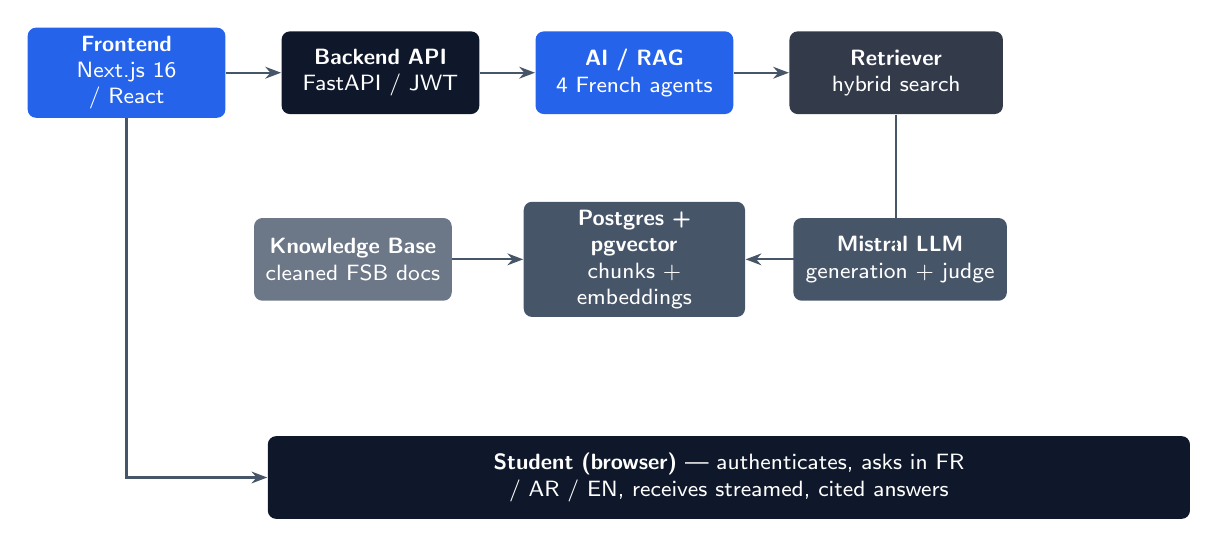
\begin{tikzpicture}[font=\sffamily\footnotesize,
  box/.style={rounded corners=3pt,draw=none,text=white,align=center,minimum height=1.05cm,inner sep=3pt},
  flow/.style={-{Stealth[length=2mm]},slate,thick}]
\node[box,fill=brandblue2,text width=2.3cm] (fe) {\textbf{Frontend}\\Next.js 16 / React};
\node[box,fill=navy,text width=2.3cm,right=0.7cm of fe] (be) {\textbf{Backend API}\\FastAPI / JWT};
\node[box,fill=brandblue2,text width=2.3cm,right=0.7cm of be] (rag) {\textbf{AI / RAG}\\4 French agents};
\node[box,fill=navy!85,text width=2.5cm,right=0.7cm of rag] (ret) {\textbf{Retriever}\\hybrid search};
\node[box,fill=slate,text width=2.6cm,below=1.1cm of rag] (pg) {\textbf{Postgres + pgvector}\\chunks + embeddings};
\node[box,fill=slate,text width=2.5cm,right=0.6cm of pg] (ml) {\textbf{Mistral LLM}\\generation + judge};
\node[box,fill=slate!80,text width=2.3cm,left=0.7cm of pg,xshift=-0.2cm] (kb) {\textbf{Knowledge Base}\\cleaned FSB docs};
\node[box,fill=navy,text width=11.5cm,below=1.5cm of pg,xshift=1.2cm] (user) {\textbf{Student (browser)} --- authenticates, asks in FR / AR / EN, receives streamed, cited answers};
\draw[flow] (fe) -- (be); \draw[flow] (be) -- (rag); \draw[flow] (rag) -- (ret);
\draw[flow] (ret) |- (ml); \draw[flow] (ret) |- (pg);
\draw[flow] (kb) -- (pg);
\draw[flow] (fe.south) |- (user.west);
\end{tikzpicture}
\caption{High-level architecture of the Digital Campus platform.}
\end{figure}

\subsection{Feature summary}
\begin{itemize}
\item \textbf{Authentication and onboarding} --- register, email verification, login (JWT), and a guided onboarding flow that sets the student profile.
\item \textbf{Chat assistant} --- streamed, token-by-token answers with inline citations to the source document and page; conversation history; and thumbs up/down feedback.
\item \textbf{Dashboard} --- the student's real profile, courses, materials and recent conversations.
\item \textbf{Courses and Google Classroom} --- add courses, upload materials (PDF/DOCX/TXT), or import them read-only from Google Classroom; imported content is scoped privately to that student.
\item \textbf{Knowledge base} --- official FSB documents cleaned, chunked, catalogued and embedded for retrieval.
\end{itemize}

% ================= 3 =================
\section{Team Organization and Work Distribution}
We worked in an \textbf{Agile / Scrum} style across two main sprints plus a final integration and hardening phase. \textbf{Aymen Jeddou} acted as \textbf{Scrum Master}, coordinating the backlog, and --- because the four areas advanced in parallel --- also owned the \textbf{integration} of everyone's branches into a single working \texttt{develop} branch. The project blueprint (\texttt{docs/FSB\_Nexus\_Blueprint.tex}) defined four roles, each owning a complete, demonstrable outcome; the team then assigned members to roles.

\subsection{Responsibility matrix}
\begin{tabularx}{\textwidth}{@{}p{4.6cm} p{3.8cm} Y@{}}
\toprule
\textbf{Blueprint role} & \textbf{Owner(s)} & \textbf{Main deliverable}\\
\midrule
Role 1 --- Conversational Intelligence \& Retrieval & Aymen Jeddou & The 4-agent RAG pipeline, retrieval quality, and the evaluation benchmark\\
Knowledge Base & Iheb Bouali & Harvested, cleaned, chunked and catalogued FSB documents\\
Role 2 --- Courses \& Integrations & Abderrahim Neji & Courses module + Google Classroom OAuth import + file upload ingestion\\
Role 3 --- Frontend \& Experience & M. A. Trabelsi (design), Iheb Bouali (enhancement) & Next.js auth, dashboard and chat UI; refreshed design in \texttt{better\_front}\\
Role 4 --- Backend, Security \& Platform & Abderrahim Neji (core API), M. A. Trabelsi (security) & FastAPI auth/profile/chat/documents, streaming endpoint, hardening\\
Scrum \& Integration & Aymen Jeddou & Backlog coordination and merging all branches into \texttt{develop}\\
\bottomrule
\end{tabularx}

\subsection{Per-member contributions}
\textbf{Aymen Jeddou --- RAG intelligent system, Scrum Master, integration.} Designed and built the agentic RAG pipeline (pull requests \#7, \#11), integrated it end-to-end with the backend and ingestion (\#16), and led a second data/quality sprint that fixed retrieval and over-refusal and added an evaluation harness (\#19). As Scrum Master he coordinated the team and personally merged the backend, courses and frontend branches into \texttt{develop}, resolving conflicts and closing quality gaps found during integration. Chapters 5 and 6 detail this work.

\textbf{Iheb Bouali --- knowledge base and frontend enhancement.} Built the knowledge base: harvested official FSB documents, then cleaned, chunked and catalogued them into the pipeline that feeds retrieval (\#9, \#14). He also enhanced the frontend on the \texttt{better\_front} branch, refining the design and user experience. (Some of this work appears under a second account, \texttt{o-MrNobody-o}.)

\textbf{Abderrahim Neji --- backend and integrations.} Implemented the core backend (authentication, profile, chat and documents endpoints, and all associated tests; \#10), then built the Courses \& Integrations module (\#20): a manual course/material path plus a read-only Google Classroom import using OAuth 2.0 with encrypted token storage and file-upload ingestion.

\textbf{Mohamed Amine Trabelsi --- frontend design, then security and platform.} Delivered the first frontend sprint (authentication, dashboard and chat UI, light/dark theme; \#12, \#13), then shifted to Role 4 and implemented backend security and platform upgrades --- including the streaming response endpoint, a feedback model, and hardening measures (\#18).

\subsection{Branch and integration workflow}
Each role worked on its own feature branch and opened a pull request. Aymen reviewed and merged them into \texttt{develop}. Integration was not a rubber stamp: for example, the streaming endpoint initially bypassed the RAG safety path (groundedness grading, intent routing and conversation memory), which was caught and rewired during integration so that streamed answers carry the same protections as non-streamed ones.

\begin{tabularx}{\textwidth}{@{}p{2.9cm} p{2.2cm} Y p{2.6cm}@{}}
\toprule
\textbf{Pull request} & \textbf{Author} & \textbf{Area} & \textbf{Merged into}\\
\midrule
\#7, \#11 & Aymen & RAG generation pipeline (agents, prompts, LLM) & develop\\
\#9, \#14 & Iheb & Knowledge base import / clean / chunk & develop\\
\#10 & Abderrahim & Backend: auth, profile, chat, documents & develop\\
\#12, \#13 & Amin & Frontend Sprint 1: auth, dashboard, chat UI & develop\\
\#16, \#17 & Aymen & End-to-end RAG integration; Sprint-1 consolidation & develop / main\\
\#18 & Amin & Role 4: security, streaming endpoint, platform & develop\\
\#19 & Aymen & KB sprint 2: retrieval + eval harness & develop\\
\#20 & Abderrahim & Courses \& Google Classroom integration & develop\\
\#21 (\texttt{better\_front}) & Iheb / Aymen & Frontend redesign + streaming/courses UI & develop\\
\bottomrule
\end{tabularx}

% ================= 4 =================
\section{Technical Architecture}
\subsection{Frontend (Next.js) --- Amin, then Iheb}
The frontend is a \textbf{Next.js 16} application (App Router, Turbopack) styled with Tailwind CSS and animated with Framer Motion. It provides authentication screens, a dashboard, a courses screen, and the chat interface. The chat consumes the backend's \textbf{Server-Sent Events (SSE)} stream to render answers token-by-token, showing citation chips beneath each reply. Light and dark themes are supported through semantic design tokens.

\subsection{Backend (FastAPI) --- Abderrahim, hardened by Amin}
The backend is a \textbf{FastAPI} REST API using JWT authentication. It exposes authentication (register / verify / login), profile and onboarding, chat (send, stream, sessions, messages, feedback), documents, and courses endpoints. Passwords are hashed; protected routes require a bearer token. Later hardening added a streaming endpoint, a login rate limiter backed by Redis, and structured logging.

\subsection{AI / RAG pipeline --- Aymen}
The heart of the platform is a set of \textbf{four specialised French-language agents} (Orientation, Academic, Administrative, Learning). A question is routed to the right agent, which runs the pipeline: \textbf{retrieve} candidate passages, \textbf{filter} them, \textbf{generate} a grounded answer with the LLM, \textbf{format citations} as \texttt{[document, p.X]}, and \textbf{grade groundedness} (a second LLM check that the answer is supported by the sources). The LLM client is provider-agnostic (Mistral by default).

\subsection{Knowledge base --- Iheb}
Official FSB documents are harvested and passed through a cleaning and chunking pipeline that splits them into passages, attaches metadata (source document, page, category), and embeds each chunk with a multilingual sentence-transformer model (768-dimensional vectors) into the \texttt{document\_chunks} table. Global knowledge-base chunks are visible to everyone; course-material chunks are scoped to a single student.

\subsection{Courses and Google Classroom --- Abderrahim}
Students can add a course and attach materials manually (typed text or an uploaded PDF/DOCX/TXT), or connect Google Classroom to import courses and materials \textbf{read-only}. The integration uses the OAuth 2.0 authorization-code flow with five read-only Classroom/Drive scopes; the callback authenticates the student via a signed \texttt{state} token, and access/refresh tokens are encrypted at rest. Imported materials are ingested into the same retrieval store, scoped to that student.

% ================= 5 =================
\section{The RAG Intelligent System in Depth}
The first working assistant was \textit{too} cautious: it refused almost every question, and when it did answer, retrieval often failed to surface passages that were actually present in the knowledge base. This chapter summarises how the system was measured and improved.

\subsection{Evaluation harness}
To improve retrieval without guessing, we built an \textbf{evaluation harness} with a labelled set of questions (\texttt{golden.jsonl}) and a larger 100-question set. It measures retrieval quality (\textbf{hit@5}, \textbf{MRR}, \textbf{recall@10}) and, with the real LLM, end-to-end quality (\textbf{answer rate}, \textbf{answer-with-citation rate}, and \textbf{false-answer rate} --- how often the assistant invents an answer to an impossible question). This benchmark served as the shared quality bar for the whole team.

\subsection{Key improvements}
\begin{itemize}
\item \textbf{Index / probe fix} --- the vector index scanned only one cluster, missing exact matches; scanning every cluster restored recall at negligible cost.
\item \textbf{Softened prompts + intent routing} --- the agents stopped refusing partial-but-useful answers, and greetings/meta questions are answered directly instead of going through retrieval.
\item \textbf{Licence and master fact cards} --- curated, well-formed entries so programme questions reliably retrieve the right card at rank 1.
\item \textbf{Hybrid retrieval} --- combining semantic (vector) search with PostgreSQL full-text search via reciprocal-rank fusion, so both meaning and exact keywords are found.
\item \textbf{Conversation memory} --- recent turns are fed back so short follow-ups still retrieve the right documents.
\item \textbf{Groundedness grader} --- a second LLM check blocks answers the sources do not support.
\end{itemize}

\subsection{Measured results}
Each change was measured against the benchmark. The table shows the progression from the strict starting point to the final integrated system.

\begin{center}
\begin{tabular}{@{}l cccc@{}}
\toprule
\textbf{Configuration} & \textbf{hit@5} & \textbf{MRR} & \textbf{answer rate} & \textbf{false answer}\\
\midrule
Starting point (strict prompt, single-probe index) & 0.50 & 0.395 & 0.60 & 0.00\\
+ index fix & \textbf{0.80} & 0.612 & 0.60 & 0.00\\
+ softened prompts \& intent routing & 0.80 & 0.612 & \textbf{0.70} & 0.00\\
+ licence fact cards & 0.80 & 0.678 & --- & ---\\
+ hybrid retrieval & \textbf{0.90} & 0.750 & \textbf{0.833} & 0.00\\
+ master cards \& memory (final) & \textbf{0.90} & \textbf{0.776} & \textbf{0.833} & 0.00--0.09\\
\bottomrule
\end{tabular}
\end{center}

Retrieval hit@5 rose from \textbf{0.50 to 0.90} and recall@10 reached \textbf{0.967}; ranking quality (MRR) nearly doubled to \textbf{0.776}. Crucially, \textbf{every answered question carries citations} (citation rate equals answer rate), so the gain is real sourced answers, not vague hedging. In the final production sprint a routing fix took the answer rate to effectively \textbf{1.0} on the reliability set.

% ================= 6 =================
\section{Final Production-Readiness Sprint}
A closing sprint made the platform demonstrable and safe to pilot. The changes below were implemented and merged to \texttt{develop}.
\begin{itemize}
\item \textbf{Streaming that actually renders} --- the chat had stalled on a loading state because the browser parsed Server-Sent Events with the wrong delimiter; fixing the parser made answers stream live with their citations.
\item \textbf{Latency} --- warming the embedding model and language-model clients at startup, plus caching, cut cold responses dramatically and gave a fast first token.
\item \textbf{Real dashboard and identity} --- the dashboard, header and sidebar now show the signed-in student's real profile, courses and conversations instead of placeholder mock data, with a logout action.
\item \textbf{Onboarding and the Academic agent} --- a new onboarding endpoint is the only way to become an \textit{enrolled} student, which unlocked the previously unreachable Academic agent; a multi-run probe confirmed it answers (0 refusals over 9 runs) rather than over-refusing.
\item \textbf{Security hardening} --- a server-side route guard redirects unauthenticated requests before any page is sent; the login rate limiter was switched on with Redis (a burst of bad logins now returns HTTP 429); and structured, timestamped logging was configured.
\item \textbf{Migrations and CI} --- the database schema is now versioned with Alembic, and a GitHub Actions pipeline runs the AI suite (43 tests) and the backend suite (26 tests) on every push and pull request.
\end{itemize}

\begin{callout}
Alongside the platform, two companion documents were produced: a changes \& deployment guide, and this report. The deployment guide covers local setup, the Google Cloud setup for Google Classroom, and a step-by-step Google Cloud deployment.
\end{callout}

% ================= 7 =================
\section{Testing and Quality Assurance}
\begin{itemize}
\item \textbf{AI / RAG unit tests (43)} --- cover retrieval delegation, citation formatting, the groundedness grader and the pipeline, with the language model mocked (no external calls).
\item \textbf{Backend API tests (26)} --- exercise the real register / verify / login flow, protected routes, chat persistence, document upload and the courses/Classroom endpoints.
\item \textbf{Evaluation harness} --- the retrieval and end-to-end metrics of Section 5, used as the shared quality benchmark.
\item \textbf{Continuous integration} --- both suites run automatically on GitHub Actions against a PostgreSQL+pgvector service after applying the Alembic migration.
\end{itemize}

% ================= 8 =================
\section{Deployment}
\textbf{Locally}, the stack runs with Docker (PostgreSQL + Redis), a shared Python environment for the backend and AI packages, and a Node environment for the frontend; the schema is created with \texttt{alembic upgrade head} and the knowledge base is ingested once.

\textbf{On Google Cloud}, the recommended path is Cloud SQL for PostgreSQL (with the \texttt{vector} extension), Memorystore for Redis, and two Cloud Run services (backend and frontend), with secrets in Secret Manager. The Google Classroom integration requires enabling the Classroom and Drive APIs, configuring the OAuth consent screen with the five read-only scopes, and registering the backend's callback URL. Full commands are in the companion deployment guide.

% ================= 9 =================
\section{Challenges and Lessons Learned}
\begin{itemize}
\item \textbf{Parallel work needs firm interfaces.} Agreeing the chat/streaming contract up front let the four roles progress independently --- but integration still surfaced gaps (the streaming path that skipped the safety checks) that only a careful merge caught.
\item \textbf{Measure before optimising.} The retrieval gains came from the evaluation harness, not intuition; the numbers showed which change actually helped.
\item \textbf{Refusing well is a feature.} An assistant that says ``I don't have that in the documents'' is more trustworthy than one that guesses; balancing this against over-refusal was a central theme.
\item \textbf{Latency is part of the correctness of the experience.} A correct answer that never renders, or takes 30 seconds, is a failure to the user; warmup and streaming addressed this.
\end{itemize}

% ================= 10 =================
\section{Conclusion and Future Work}
Over the summer 2026 internship the team delivered a working, source-grounded academic assistant for the FSB: a polished frontend, a secure backend, a measured and reliable RAG pipeline, a real knowledge base, and a courses integration --- unified on the \texttt{develop} branch and ready for a final review before merging to \texttt{main}.

\textbf{Future work} (deferred for a later hardening pass): migrate the session to httpOnly cookies and add refresh tokens and password reset; wire real email (SMTP) for verification; complete Google's OAuth verification for public Classroom use; and broaden the evaluation set to cover course-content questions.

% ================= APPENDIX =================
\appendix
\section{Technology Stack}
\begin{tabularx}{\textwidth}{@{}p{3.2cm} Y@{}}
\toprule
\textbf{Layer} & \textbf{Technologies}\\
\midrule
Frontend & Next.js 16 (App Router), React, TypeScript, Tailwind CSS, Framer Motion\\
Backend & FastAPI, SQLAlchemy, JWT, Alembic, Redis (rate limiting)\\
AI / RAG & Python, Mistral LLM (provider-agnostic client), sentence-transformers embeddings\\
Data & PostgreSQL + pgvector; hybrid vector + full-text retrieval\\
Integrations & Google Classroom \& Drive (OAuth 2.0, read-only)\\
Platform & Docker Compose, GitHub Actions CI, Google Cloud (Cloud Run, Cloud SQL, Memorystore)\\
\bottomrule
\end{tabularx}

\section{Repository, Branches and Pull Requests}
All work is on the \texttt{develop} branch of the team's GitHub repository. Key feature branches: \texttt{feature/rag-pipeline}, \texttt{feature/kb-sprint2}, \texttt{feature/backend}, \texttt{amine-backend}, \texttt{courses-and-integrations}, \texttt{feature/frontend}, \texttt{better\_front}. Pull requests \#7--\#21 record the detailed history and reviews.

\end{document}
